\documentclass[11pt]{article}

% Same look as the base paper: Computer Modern, US letter, 1 inch margins.
\usepackage[letterpaper,margin=1in]{geometry}
\usepackage[T1]{fontenc}
\usepackage{amsmath,amssymb}
\usepackage{graphicx}
\usepackage{booktabs}
\usepackage{caption}
\usepackage{xcolor}
\usepackage{tikz}
\usetikzlibrary{arrows.meta,positioning,decorations.pathreplacing,calc}
\usepackage[section]{placeins}   % every figure stays inside its own section
\usepackage[hidelinks]{hyperref}

% A figure-heavy paper: let LaTeX fill pages with floats instead of pushing them to the end.
\renewcommand{\topfraction}{0.9}
\renewcommand{\bottomfraction}{0.8}
\renewcommand{\textfraction}{0.07}
\renewcommand{\floatpagefraction}{0.75}
\setcounter{topnumber}{3}
\setcounter{bottomnumber}{2}
\setcounter{totalnumber}{5}

\captionsetup{font=small,labelfont=bf}
\graphicspath{{figures/}}

% Colour roles shared with the Python figures (code/asmm/style.py).
\definecolor{asblue}{HTML}{2A78D6}
\definecolor{asdark}{HTML}{174A8A}
\definecolor{symorange}{HTML}{EB6834}
\definecolor{ink}{HTML}{0B0B0B}
\definecolor{ink2}{HTML}{52514E}
\definecolor{holds}{HTML}{008300}
\definecolor{breaks}{HTML}{E34948}

% Generated by code/run_all.py. Do not edit.
\newcommand{\GammaRA}{0.005}
\newcommand{\Horizon}{360}
\newcommand{\CalibDays}{10}
\newcommand{\Paths}{10,000}
\newcommand{\RELIANCEDays}{19}
\newcommand{\RELIANCETestDays}{9}
\newcommand{\RELIANCESigma}{0.676}
\newcommand{\RELIANCEA}{1.49}
\newcommand{\RELIANCEk}{2.52}
\newcommand{\RELIANCERTwo}{0.984}
\newcommand{\RELIANCEAcfOne}{-0.014}
\newcommand{\RELIANCEVRfifteen}{0.90}
\newcommand{\RELIANCESigmaRatio}{3.1}
\newcommand{\RELIANCEKurt}{10.9}
\newcommand{\RELIANCEAmihud}{7.18e-06}
\newcommand{\RELIANCERoll}{0.37}
\newcommand{\RELIANCENoTrade}{0.2}
\newcommand{\RELIANCEVarqAS}{12.0}
\newcommand{\RELIANCEVarqSym}{231.7}
\newcommand{\RELIANCEVarqFactor}{19}
\newcommand{\RELIANCEVarqTheory}{233.7}
\newcommand{\RELIANCECEAS}{122.8}
\newcommand{\RELIANCECESym}{82.7}
\newcommand{\RELIANCECEciLo}{34.3}
\newcommand{\RELIANCECEciHi}{46.2}
\newcommand{\RELIANCEMeanAS}{123.4}
\newcommand{\RELIANCEMeanSym}{139.0}
\newcommand{\RELIANCEHalfSpread}{0.60}
\newcommand{\RELIANCEReplayPnlAS}{-24.1}
\newcommand{\RELIANCEReplayPnlSym}{-78.0}
\newcommand{\RELIANCEReplaySdAS}{22.5}
\newcommand{\RELIANCEReplaySdSym}{108.8}
\newcommand{\RELIANCEReplaySdFactor}{4.8}
\newcommand{\RELIANCEReplayAbsqAS}{0.7}
\newcommand{\RELIANCEReplayAbsqSym}{6.7}
\newcommand{\RELIANCECaptureAS}{+135.2}
\newcommand{\RELIANCEAdverseAS}{-163.1}
\newcommand{\RELIANCECarryAS}{+3.7}
\newcommand{\RELIANCEReplayCEAS}{-25.3}
\newcommand{\RELIANCEReplayCESym}{-102.2}
\newcommand{\RELIANCEAllSdFactor}{6.3}
\newcommand{\RELIANCEAllPnlAS}{-19.2}
\newcommand{\RELIANCEAllPnlSym}{-55.9}
\newcommand{\RELIANCESpreadOpen}{1.62}
\newcommand{\RELIANCESpreadMid}{1.20}
\newcommand{\KSCLDays}{19}
\newcommand{\KSCLTestDays}{9}
\newcommand{\KSCLSigma}{0.863}
\newcommand{\KSCLA}{0.84}
\newcommand{\KSCLk}{1.81}
\newcommand{\KSCLRTwo}{0.992}
\newcommand{\KSCLAcfOne}{-0.123}
\newcommand{\KSCLVRfifteen}{0.65}
\newcommand{\KSCLSigmaRatio}{3.2}
\newcommand{\KSCLKurt}{99.4}
\newcommand{\KSCLAmihud}{2.35e-03}
\newcommand{\KSCLRoll}{0.69}
\newcommand{\KSCLNoTrade}{8.8}
\newcommand{\KSCLVarqAS}{8.5}
\newcommand{\KSCLVarqSym}{119.7}
\newcommand{\KSCLVarqFactor}{14}
\newcommand{\KSCLVarqTheory}{121.2}
\newcommand{\KSCLCEAS}{92.9}
\newcommand{\KSCLCESym}{59.9}
\newcommand{\KSCLCEciLo}{28.1}
\newcommand{\KSCLCEciHi}{38.4}
\newcommand{\KSCLMeanAS}{93.6}
\newcommand{\KSCLMeanSym}{107.4}
\newcommand{\KSCLHalfSpread}{0.89}
\newcommand{\KSCLReplayPnlAS}{-28.9}
\newcommand{\KSCLReplayPnlSym}{+38.7}
\newcommand{\KSCLReplaySdAS}{19.4}
\newcommand{\KSCLReplaySdSym}{141.6}
\newcommand{\KSCLReplaySdFactor}{7.3}
\newcommand{\KSCLReplayAbsqAS}{0.5}
\newcommand{\KSCLReplayAbsqSym}{6.6}
\newcommand{\KSCLCaptureAS}{+80.1}
\newcommand{\KSCLAdverseAS}{-128.2}
\newcommand{\KSCLCarryAS}{+19.3}
\newcommand{\KSCLReplayCEAS}{-29.8}
\newcommand{\KSCLReplayCESym}{-4.8}
\newcommand{\KSCLAllSdFactor}{7.5}
\newcommand{\KSCLAllPnlAS}{-27.8}
\newcommand{\KSCLAllPnlSym}{-7.9}
\newcommand{\KSCLSpreadOpen}{2.45}
\newcommand{\KSCLSpreadMid}{1.78}
   % every number cited in the text, generated by code/run_all.py

\title{Does Optimal Market Making Survive\\ the National Stock Exchange?\\[4pt]
\large Calibrating and Testing the Avellaneda--Stoikov Model on Indian Equities}
\author{Aaryan Pradhan (22CH3FP25) \and Suhani Kumari (22CH3FP16) \and Md Arsh Ansari (22CH3FP20)\\[6pt]
\small BM51002 Market Microstructure, Term Project\\
\small Vinod Gupta School of Management, Indian Institute of Technology Kharagpur}
\date{}

\begin{document}
\maketitle

\begin{abstract}
\noindent The Avellaneda--Stoikov (2008) model tells a dealer where to quote when every fill adds to a
risky inventory, and simulation studies, including the one this project builds on, show it controls
that risk well. None of them test it on real order flow. We take the model to the National Stock
Exchange of India. Using \RELIANCEDays{} days of one-minute bars for a liquid stock (RELIANCE) and an
illiquid one (KSCL), we test each assumption, calibrate the volatility $\sigma$ and the fill-intensity
curve $Ae^{-k\delta}$, and run the optimal quotes twice: in the model's own world (a
\Paths-path Monte Carlo) and on the real minutes (an out-of-sample historical replay against a
symmetric dealer quoting the same average spread). The central assumption holds: fill intensity
decays exponentially in the quote distance ($R^2 \ge \RELIANCERTwo$). The illiquid stock's mid-price
shows the Roll bid--ask bounce, and intraday volatility varies by a factor of about three, so
those assumptions bend or break. On real data the model's inventory control survives: it cuts
the standard deviation of daily PnL by a factor of \RELIANCEReplaySdFactor{} (RELIANCE) and
\KSCLReplaySdFactor{} (KSCL) and keeps inventory near zero. Its profit does not survive: an exact
decomposition shows adverse selection, which the model assumes away, consumes the whole spread
income. The model's optimal spread is also several times the market's Roll spread, which is what a
monopolist dealer facing a competitive limit order book should expect. We conclude that
Avellaneda--Stoikov works on NSE as a risk-control rule, not as a stand-alone source of profit.
\end{abstract}

\noindent\textbf{\textit{Keywords:}} Market making; Inventory risk; Avellaneda--Stoikov;
National Stock Exchange; Fill intensity; Adverse selection; Roll spread; Amihud illiquidity

\section{Introduction}

\subsection{The Question}

A market maker earns the bid--ask spread, but the two sides of a trade do not arrive together.
A dealer who is filled on the bid first is long the stock until someone lifts the ask, and every
minute spent holding that position is exposed to the price. The inventory models of
Garman~\cite{garman1976}, Amihud and Mendelson~\cite{amihudmendelson1980}, Stoll~\cite{stoll1978} and
Ho and Stoll~\cite{hostoll1981} all answer the same question: how should a dealer set prices when
inventory is risky? Avellaneda and Stoikov~\cite{avellaneda2008} restate the answer for a modern
limit order book. Their dealer shifts both quotes away from the side it is already heavy on, and
the size of the shift grows with inventory, risk aversion, volatility and the time left in the
session.

The working paper this project builds on~\cite{amargos2026} derives the model in full and confirms
in a Monte Carlo study that this skew cuts terminal-inventory variance by about an order of
magnitude. Its own scope section is explicit about what it does not do: it \emph{``does not
calibrate or backtest the model against live order-book data''}. That gap is the starting point
here. We ask one question:

\begin{center}
\emph{Does the Avellaneda--Stoikov model survive contact with the National Stock Exchange of India?}
\end{center}

\noindent ``Survive'' has three concrete meanings, and the paper answers them in order.
\begin{enumerate}
\item \textbf{Do its assumptions hold on NSE data?} We test each one and sort it into
  \emph{holds}, \emph{bends} or \emph{breaks}.
\item \textbf{Does its risk control carry over?} We compare the optimal quotes with a symmetric
  dealer quoting the same average spread, first in the model's own world, then on real minutes.
\item \textbf{Does its profit carry over, and is its spread close to the market's?} We split the
  dealer's real PnL into spread capture, adverse selection and inventory carry, and we compare the
  model's spread with the Roll~\cite{roll1984} spread the market actually charges.
\end{enumerate}

\subsection{What We Find}

Figure~\ref{fig:roadmap} summarises the argument. The model's core assumption, that fills
arrive at a rate $Ae^{-k\delta}$ decaying exponentially in the quote distance $\delta$, holds
remarkably well for both stocks. Its picture of the mid-price bends for the illiquid stock,
which shows the bid--ask bounce Roll described, and breaks on intraday volatility, which is
U-shaped rather than constant. In the model's world the optimal quotes beat the symmetric
dealer on every risk measure. On real NSE minutes the risk result survives almost intact, but
the profit result does not: fills on a real exchange carry information, so the price tends to
keep moving against the dealer after each fill, and this adverse selection eats all of the
spread income. The market's own spread is far narrower than the model's, which is what one
expects when a single dealer's optimum is set against a book full of competing liquidity
providers.

\begin{figure}[!htbp]
\centering
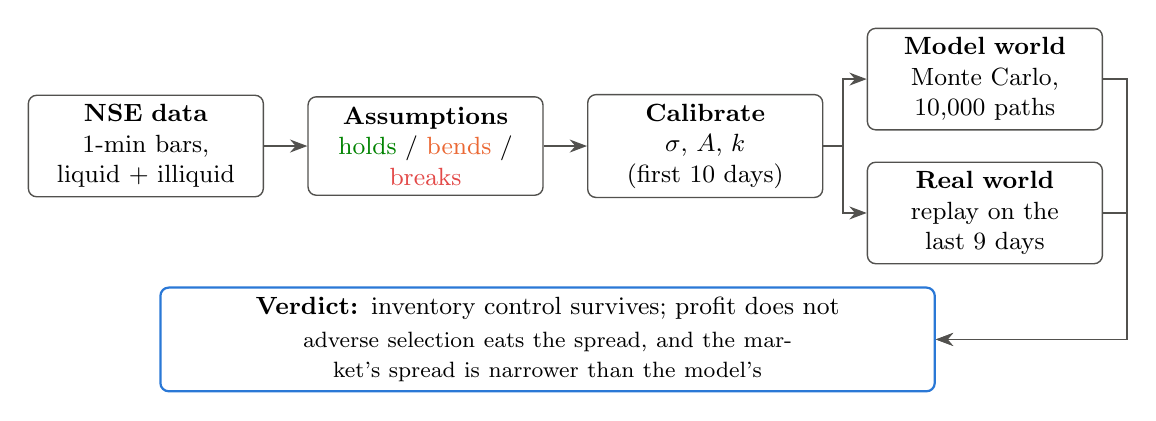
\begin{tikzpicture}[
  box/.style={draw=ink2, rounded corners=3pt, align=center, font=\small, minimum height=1.25cm,
              text width=2.75cm, fill=white, line width=0.5pt},
  arr/.style={-{Stealth[length=2.2mm]}, ink2, line width=0.6pt},
  node distance=0.55cm]
  \node[box] (data) {\textbf{NSE data}\\ 1-min bars,\\ liquid + illiquid};
  \node[box, right=of data] (test) {\textbf{Assumptions}\\
    {\color{holds}holds} / {\color{symorange}bends} /\\ {\color{breaks}breaks}};
  \node[box, right=of test] (cal) {\textbf{Calibrate}\\ $\sigma$, $A$, $k$\\ (first \CalibDays{} days)};
  \node[box, right=of cal, yshift=0.85cm] (mc) {\textbf{Model world}\\ Monte Carlo,\\ \Paths{} paths};
  \node[box, right=of cal, yshift=-0.85cm] (rp) {\textbf{Real world}\\ replay on the\\ last 9 days};
  \node[box, below=1.15cm of test, xshift=1.55cm, text width=9.6cm, minimum height=1.0cm, draw=asblue, line width=0.8pt] (verdict)
    {\textbf{Verdict:} inventory control survives; profit does not\\[1pt]
     {\footnotesize adverse selection eats the spread, and the market's spread is narrower than the model's}};
  \draw[arr] (data) -- (test);
  \draw[arr] (test) -- (cal);
  \draw[arr] (cal.east) -- ++(0.25,0) |- (mc.west);
  \draw[arr] (cal.east) -- ++(0.25,0) |- (rp.west);
  \draw[arr] (mc.east) -- ++(0.3,0) |- (verdict.east);
  \draw[arr] (rp.east) -- ++(0.3,0) |- (verdict.east);
\end{tikzpicture}
\caption{The argument of the paper. Each box is a section; each arrow is a result the next step needs.}
\label{fig:roadmap}
\end{figure}

\subsection{Organization}

Section~\ref{sec:model} states the model and the closed-form quotes we test.
Section~\ref{sec:data} describes the data and the two stocks. Section~\ref{sec:assumptions}
tests the assumptions and calibrates the parameters. Section~\ref{sec:nse} shows what the
optimal quotes look like at NSE parameters. Section~\ref{sec:mc} runs the model in its own world
and Section~\ref{sec:replay} runs it on real minutes. Section~\ref{sec:discussion} compares the
two and sets the model's spread against the market's, and Section~\ref{sec:conclusion}
concludes. The appendix documents the code and data needed to reproduce every figure.

\section{The Avellaneda--Stoikov Model}
\label{sec:model}

This section restates only what the empirical work needs. Full derivations are in
\cite{avellaneda2008} and \cite{amargos2026}.

\subsection{Setup}

Time runs over one trading session $t\in[0,T]$. We measure time in minutes, so $T=\Horizon$.
The mid-price is an arithmetic Brownian motion with no drift,
\begin{equation}
dS_t = \sigma\, dW_t ,
\label{eq:mid}
\end{equation}
where $\sigma$ is in rupees per $\sqrt{\text{minute}}$. The dealer posts a bid at $S_t-\delta^b_t$
and an ask at $S_t+\delta^a_t$, with distances $\delta^b,\delta^a\ge 0$. Market orders hit the
bid and lift the ask as two independent Poisson processes whose intensity depends only on the
distance of the quote from the mid,
\begin{equation}
\lambda(\delta) = A\,e^{-k\delta}.
\label{eq:lambda}
\end{equation}
$A$ is the fill rate of a quote sitting at the mid; $k$ is how fast that rate falls as the quote
moves away. Each fill is one share. Inventory $q_t$ is bids filled minus asks filled, cash $X_t$
moves by the fill prices, and the dealer maximises expected CARA utility of terminal wealth,
$\mathbb{E}\big[-e^{-\gamma(X_T+q_TS_T)}\big]$, with absolute risk aversion $\gamma$ in $1/\text{INR}$.

\subsection{The Optimal Quotes}

Solving the Hamilton--Jacobi--Bellman equation with the CARA ansatz gives two closed-form
objects~\cite{avellaneda2008}. The first is the \emph{reservation price}, the price at which the
dealer is indifferent to holding one more share,
\begin{equation}
r(s,q,t) = s - q\,\gamma\sigma^2 (T-t).
\label{eq:reservation}
\end{equation}
A long dealer ($q>0$) values the stock below the mid, a short dealer above it. The second is
the optimal \emph{total spread}, centred on $r$ rather than on $s$,
\begin{equation}
\delta^a+\delta^b = \underbrace{\gamma\sigma^2(T-t)}_{\text{inventory-risk premium}}
 \;+\; \underbrace{\frac{2}{\gamma}\ln\!\Big(1+\frac{\gamma}{k}\Big)}_{\text{market-making edge}} .
\label{eq:spread}
\end{equation}
The first term pays for carrying inventory risk over the time left and shrinks to zero at the
close. The second is what a dealer charges for liquidity alone; it depends only on how fast the
order book thins out ($k$). Figure~\ref{fig:schematic} draws both objects. Together they are the
whole strategy: quote $r\pm\frac12(\delta^a+\delta^b)$, floored so that neither quote crosses the
mid.

\begin{figure}[!htbp]
\centering
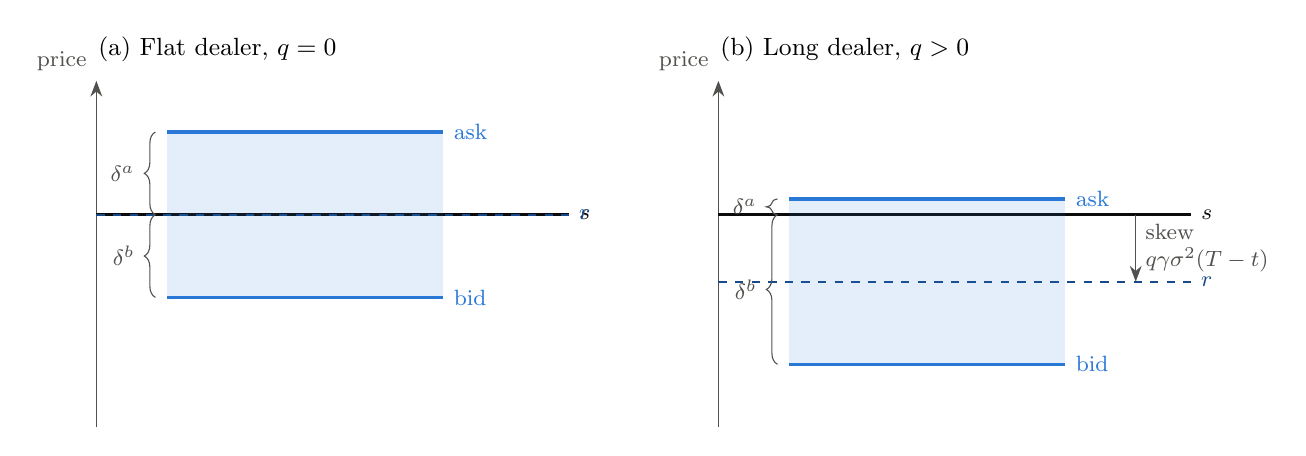
\begin{tikzpicture}[x=1cm,y=1cm,font=\small]
  \foreach \xo/\rr/\ttl in {0/2.9/{(a) Flat dealer, $q=0$}, 7.9/2.05/{(b) Long dealer, $q>0$}} {
    \begin{scope}[xshift=\xo cm]
      \node[anchor=west] at (-0.1,5.0) {\ttl};
      \draw[ink2, -{Stealth[length=2mm]}] (0,0.2) -- (0,4.6) node[above left, font=\footnotesize] {price};
      \draw[ink, line width=0.9pt] (0,2.9) -- (6.0,2.9) node[right, font=\footnotesize] {$s$};
      \draw[asdark, dashed, line width=0.8pt] (0,\rr) -- (6.0,\rr) node[right, font=\footnotesize] {$r$};
      \fill[asblue, opacity=0.13] (0.9,\rr-1.05) rectangle (4.4,\rr+1.05);
      \draw[asblue, line width=1.3pt] (0.9,\rr+1.05) -- (4.4,\rr+1.05) node[right, font=\footnotesize] {ask};
      \draw[asblue, line width=1.3pt] (0.9,\rr-1.05) -- (4.4,\rr-1.05) node[right, font=\footnotesize] {bid};
      \draw[decorate, decoration={brace, amplitude=4pt}, ink2] (0.75,2.9) -- (0.75,\rr+1.05)
        node[midway, left=4pt, font=\footnotesize] {$\delta^a$};
      \draw[decorate, decoration={brace, amplitude=4pt, mirror}, ink2] (0.75,2.9) -- (0.75,\rr-1.05)
        node[midway, left=4pt, font=\footnotesize] {$\delta^b$};
    \end{scope}
  }
  \draw[ink2, -{Stealth[length=2mm]}] (7.9+5.3,2.9) -- (7.9+5.3,2.05)
    node[midway, right, font=\footnotesize, align=left] {skew\\$q\gamma\sigma^2(T-t)$};
\end{tikzpicture}
\caption{How the optimal quotes move with inventory. (a) A flat dealer quotes symmetrically
around the mid. (b) A long dealer's reservation price falls below the mid, so the ask moves closer
(it sells more often) and the bid moves away (it buys less often). The width of the band is the
spread of equation~\eqref{eq:spread} and does not depend on $q$; only its position does.}
\label{fig:schematic}
\end{figure}

\subsection{Assumption Ledger}
\label{sec:ledger}

The base paper lists the assumptions behind these formulas. We restate the ones that real data can
test, numbered so that Section~\ref{sec:assumptions} can check each one.
\begin{enumerate}
\item[\textbf{A1}] \textbf{Exponential fill intensity:} $\lambda(\delta)=Ae^{-k\delta}$, equation~\eqref{eq:lambda}.
\item[\textbf{A2}] \textbf{Symmetric book:} the same $A$ and $k$ on the bid and the ask side.
\item[\textbf{A3}] \textbf{Driftless mid:} no predictable trend in $S_t$ over a session.
\item[\textbf{A4}] \textbf{Independent Gaussian increments:} $S_t$ is a Brownian motion, so its
  changes are uncorrelated, scale linearly in variance with the horizon, and are normal.
\item[\textbf{A5}] \textbf{Constant parameters:} $\sigma$, $A$ and $k$ do not change within
  a session or across sessions.
\item[\textbf{A6}] \textbf{No adverse selection:} a fill tells the dealer nothing about where the
  price goes next. This cannot be tested on its own; Section~\ref{sec:replay} measures its cost.
\end{enumerate}

\section{Data}
\label{sec:data}

\subsection{Source and Sample}

We use one-minute OHLCV bars (open, high, low, close, volume) from Yahoo Finance for
\RELIANCEDays{} NSE trading days, 30 September to 28 October 2026. Yahoo keeps one-minute
history for about 30 days, so this is the full window available. Two cleaning steps matter:
\begin{enumerate}
\item \textbf{Session window.} Yahoo drops the 15:16--15:27 bars and then prints a single
  catch-up bar at 15:28. Keeping that bar would create a fake volatility spike at the close.
  We use the clean window 09:15--15:14, which gives exactly $T=\Horizon$ one-minute bars per day.
\item \textbf{Minutes with no trade.} A missing bar inside the window means nobody traded that
  minute. We carry the last close forward (the mid did not move), leave the high and low empty
  (no quote could have been filled) and set volume to zero. Nothing is interpolated.
\end{enumerate}
The first \CalibDays{} days are the \emph{calibration window}; the remaining
\RELIANCETestDays{} days are held out as the \emph{test window} (Figure~\ref{fig:prices}).

\subsection{Choosing a Liquid and an Illiquid Stock}

The model's predictions depend on liquidity: a thin book means fewer fills per unit of price risk,
so inventory control should matter more. We therefore study a contrasting pair. RELIANCE is the
most heavily traded NSE large-cap. For the illiquid stock we screened twelve small-caps by
Amihud's~\cite{amihud2002} illiquidity ratio and by the share of minutes with no trade, and chose
KSCL (Kaveri Seed). It is among the most illiquid names screened, it still trades in most
minutes, and its price level is close enough to RELIANCE's that spreads in rupees are comparable.
Table~\ref{tab:descriptive} and Figure~\ref{fig:liquidity} show how far apart the two are: KSCL's
Amihud ratio is about 300 times RELIANCE's, and \KSCLNoTrade\% of its minutes have no trade.

\begin{table}[!htbp]
\centering
\caption{Descriptive statistics, all \RELIANCEDays{} days, 09:15--15:14.}
\label{tab:descriptive}
\small
\begin{tabular}{lrr}
\toprule
Statistic & RELIANCE & KSCL \\
\midrule
Trading days & 19 & 19 \\
Mean price (INR) & 1,189.3 & 712.4 \\
Mean daily traded value (INR crore) & 1,640.27 & 9.19 \\
Minutes with no trade (\%) & 0.2\% & 8.8\% \\
$\sigma$, one-minute price change (INR) & 0.823 & 1.001 \\
Mean one-minute high--low range (INR) & 1.020 & 0.655 \\
Amihud ILLIQ ($|R|$ per INR crore) & 7.18e-06 & 2.35e-03 \\
Roll spread (INR) & 0.373 & 0.686 \\
\bottomrule
\end{tabular}

\end{table}

\begin{figure}[!htbp]
\centering
\includegraphics[width=\textwidth]{data_price_paths}
\caption{One-minute closing prices, all sessions placed end to end (thin vertical lines separate
days). The shaded part is the calibration window; the model is tested only on the unshaded days.}
\label{fig:prices}
\end{figure}

\begin{figure}[!htbp]
\centering
\includegraphics[width=\textwidth]{data_liquidity}
\caption{Daily liquidity. (a) Amihud~\cite{amihud2002} illiquidity, $|R_d|$ per crore of traded
value (log scale): KSCL is two to three orders of magnitude less liquid. (b) Roll~\cite{roll1984}
spread, $2\sqrt{-\mathrm{Cov}(\Delta p_t,\Delta p_{t-1})}$; the measure is undefined (gaps) on days
when the covariance is positive, which happens often for RELIANCE. (c) Share of minutes with no
trade.}
\label{fig:liquidity}
\end{figure}

\subsection{The Trading Day Is Not Uniform}

Figure~\ref{fig:volume} shows the familiar intraday U-shape~\cite{admati1988}: trading is heaviest
at the open and in the last half hour. KSCL's curve is noisier and has bursts in the middle of the
day, typical of a stock where a few large orders dominate volume. This pattern matters for the
model, which assumes order flow and volatility are constant through the session (A5).

\begin{figure}[!htbp]
\centering
\includegraphics[width=\textwidth]{data_intraday_volume}
\caption{Average share of daily volume traded in each minute (thin: raw; thick: 9-minute moving
average). The dashed line is a perfectly uniform day.}
\label{fig:volume}
\end{figure}

\section{Do the Assumptions Hold? Calibration and Tests}
\label{sec:assumptions}

\subsection{Measuring Fill Intensity from Bars}

Bars do not show the order book, so we infer fills from price excursions. Suppose that at the end
of minute $t$ a dealer posts an ask at $S_t+\delta$, where $S_t$ is the close. The ask is
\emph{filled} if the next minute's high reaches it, $H_{t+1}\ge S_t+\delta$; the bid at
$S_t-\delta$ is filled if $L_{t+1}\le S_t-\delta$. For each distance $\delta$ on a grid we count the
fraction $p(\delta)$ of minutes with a fill. If fills arrive as a Poisson process with intensity
$\lambda(\delta)$, the probability of at least one fill in one minute is $1-e^{-\lambda(\delta)}$, so
\begin{equation}
\lambda(\delta) = -\ln\big(1-p(\delta)\big), \qquad
\ln\lambda(\delta) = \ln A - k\,\delta .
\label{eq:fit}
\end{equation}
Under A1 the points $(\delta,\ln\lambda)$ lie on a straight line, and an ordinary least-squares fit
gives $\ln A$ as the intercept and $-k$ as the slope. We fit only distances with
$0.02<p(\delta)<0.98$, where $p$ is estimated precisely. The volatility $\sigma$ is the standard
deviation of one-minute changes in the close. All three are estimated on the calibration window
only. A synthetic test in the code checks that this procedure recovers known values of $A$ and $k$
to within 3\%.

\subsection{A1--A2: Fill Intensity Is Exponential and Symmetric}

\begin{figure}[!htbp]
\centering
\includegraphics[width=\textwidth]{calib_fill_curves}
\caption{The model's central assumption, tested. Implied fill intensity $\lambda(\delta)$ against
quote distance on a log scale, calibration window. Filled circles: ask side; open squares: bid side;
grey points lie outside the fitting band. A straight line on this scale is exactly
$\lambda=Ae^{-k\delta}$.}
\label{fig:fill}
\end{figure}

Figure~\ref{fig:fill} is the central test of the paper, and the answer is clear. On a log scale
the points lie on a straight line for both stocks and both sides of the book, with
$R^2\ge\RELIANCERTwo$ for RELIANCE and $R^2\ge\KSCLRTwo$ for KSCL (Table~\ref{tab:calibration}).
The two sides give nearly the same slope ($k_{\text{bid}}/k_{\text{ask}}$ within 10\%), so one
curve for both sides (A2) is a fair simplification. The liquid stock has the higher $A$ (more fills
at any distance) and the higher $k$ (its book thins out faster, because competing quotes sit close
to the mid).

The residuals in Figure~\ref{fig:residuals} show where the fit is imperfect. They curve gently
upward at both ends: quotes at the mid are filled a little more often than the line predicts,
and so are quotes far away. The tail of real fill intensity is therefore slightly fatter than
exponential, consistent with occasional large orders sweeping several price levels. The
deviations are small: apart from the single point at $\delta=0$, they stay within about 0.25 in log units, so A1 holds.

\begin{figure}[!htbp]
\centering
\includegraphics[width=\textwidth]{calib_fill_residuals}
\caption{Residuals of the log-linear fit (circles: ask, squares: bid). The gentle upward curve at
both ends means real fills have a slightly fatter tail than $e^{-k\delta}$.}
\label{fig:residuals}
\end{figure}

\begin{table}[!htbp]
\centering
\caption{Calibrated parameters, first \CalibDays{} days. The model uses one curve for both sides,
so $A$ and $k$ are averaged over the bid and the ask.}
\label{tab:calibration}
\small
\begin{tabular}{lrr}
\toprule
Parameter & RELIANCE & KSCL \\
\midrule
$\sigma$ (INR$/\sqrt{\text{min}}$) & 0.676 & 0.863 \\
$A$ (fills per minute), ask / bid & 1.341 / 1.631 & 0.756 / 0.927 \\
$k$ (per INR), ask / bid & 2.400 / 2.636 & 1.747 / 1.863 \\
$A$ used (mean of sides) & 1.486 & 0.842 \\
$k$ used (mean of sides) & 2.518 & 1.805 \\
$R^2$ of log-linear fit, ask / bid & 0.984 / 0.989 & 0.992 / 0.995 \\
Points in fit, ask / bid & 51 / 48 & 46 / 46 \\
\bottomrule
\end{tabular}

\end{table}

\subsection{A3--A4: The Mid-Price Is Close to a Random Walk, Except for the Bounce}

The mean one-minute price change is statistically zero for both stocks, so A3 holds. A4 bends.
Figure~\ref{fig:returns} shows that one-minute changes are far from normal: excess kurtosis is
\RELIANCEKurt{} for RELIANCE and \KSCLKurt{} for KSCL, because most minutes move by zero or one tick
and a few move by many (Figure~\ref{fig:qq}). Fat tails matter little for the model, whose
formulas only use the variance $\sigma^2$.

\begin{figure}[!htbp]
\centering
\includegraphics[width=\textwidth]{data_return_distribution}
\caption{Distribution of one-minute price changes, binned in whole ticks, on a log scale, with the
normal density of the same mean and variance. The empirical tails are far heavier.}
\label{fig:returns}
\end{figure}

\begin{figure}[!htbp]
\centering
\includegraphics[width=0.56\textwidth]{data_qq}
\caption{Normal quantile--quantile plot of standardised one-minute price changes. Both stocks
leave the line beyond about two standard deviations.}
\label{fig:qq}
\end{figure}

The important departure is in the dependence of price changes. For KSCL the first-order
autocorrelation is \KSCLAcfOne{} (Figure~\ref{fig:acf}), well outside the 95\% band, while
RELIANCE's is \RELIANCEAcfOne{}. This is the bid--ask bounce of Roll~\cite{roll1984}: when the last
trade is at the ask, the next is more likely at the bid, so recorded prices zig-zag even if the
true value does not move. The variance ratio of Lo and MacKinlay~\cite{lo1988},
$\mathrm{VR}(h)=\mathrm{Var}(S_{t+h}-S_t)/\big(h\,\mathrm{Var}(S_{t+1}-S_t)\big)$, which equals one for
a random walk, tells the same story over longer horizons (Figure~\ref{fig:vr}): it falls to
\KSCLVRfifteen{} at fifteen minutes for KSCL but stays at \RELIANCEVRfifteen{} for RELIANCE. The
practical consequence is that one-minute $\sigma$ overstates the true price risk of holding KSCL
over longer horizons. The model therefore over-penalises KSCL inventory, which makes it, if anything,
more conservative.

\begin{figure}[!htbp]
\centering
\includegraphics[width=\textwidth]{diag_autocorrelation}
\caption{Autocorrelation of one-minute price changes, lags 1--10 (shaded: 95\% band under
independence). KSCL's large negative first lag is the bid--ask bounce.}
\label{fig:acf}
\end{figure}

\begin{figure}[!htbp]
\centering
\includegraphics[width=\textwidth]{diag_variance_ratio}
\caption{Variance ratio against horizon. A random walk stays on the dashed line; values below one
mean price changes partly reverse. The illiquid stock reverses much more.}
\label{fig:vr}
\end{figure}

\subsection{A5: Parameters Are Not Constant}

Volatility is the assumption that breaks. Figure~\ref{fig:sigma} shows the fifteen-minute
volatility profile: $\sigma$ in the first fifteen minutes is two to three times its midday value, and across
the day the highest bucket is \RELIANCESigmaRatio{} times the lowest for RELIANCE (\KSCLSigmaRatio{}
for KSCL). The model uses one $\sigma$ for the whole day, so it under-prices inventory risk at the
open and over-prices it at midday. Across days (Figure~\ref{fig:stability}) the parameters are
steadier but not fixed: the daily $k$ varies with a coefficient of variation of about 0.17, and the
test window is somewhat more volatile than the calibration window, a realistic handicap for an
out-of-sample test.

\begin{figure}[!htbp]
\centering
\includegraphics[width=\textwidth]{data_intraday_sigma}
\caption{(a) Volatility in each fifteen-minute bucket relative to the session average; a model with
constant $\sigma$ would be the dashed line. (b) Share of minutes with at least one trade.}
\label{fig:sigma}
\end{figure}

\begin{figure}[!htbp]
\centering
\includegraphics[width=\textwidth]{calib_stability}
\caption{Parameters re-estimated day by day. Dashed lines: the calibration-window values used in
the rest of the paper. Shaded: calibration window.}
\label{fig:stability}
\end{figure}

\subsection{Scorecard}

Table~\ref{tab:scorecard} collects the verdicts. The assumption the model is built on, the
exponential fill curve, holds. The description of the price process bends, mostly for the illiquid
stock. Constant intraday volatility breaks. None of these failures is large enough to make the
calibrated model meaningless, so we now take it to the data.

\begin{table}[!htbp]
\centering
\caption{Assumption scorecard. ``Holds'': the data match the assumption. ``Bends'': a measurable
departure that the model tolerates. ``Breaks'': a departure large enough to change the quotes.}
\label{tab:scorecard}
\small
\begin{tabular}{llrrl}
\toprule
Assumption & Statistic & RELIANCE & KSCL & Verdict \\
\midrule
Fill intensity is $Ae^{-k\delta}$ & min $R^2$ & 0.984 & 0.992 & Holds \\
One curve for both sides & $k_{\text{bid}}/k_{\text{ask}}$ & 1.10 & 1.07 & Holds \\
Mid has no drift & $t$-stat of mean change & -0.26 & -0.43 & Holds \\
Independent increments & lag-1 autocorrelation & -0.014 & -0.123 & Bends (illiquid) \\
Random-walk scaling & VR(15) & 0.90 & 0.65 & Bends (illiquid) \\
Gaussian increments & excess kurtosis & 10.9 & 99.4 & Bends \\
Constant $\sigma$ through the day & max/min 15-min $\sigma$ & 3.1 & 3.2 & Breaks \\
Constant $k$ across days & coef.\ of variation of daily $k$ & 0.17 & 0.18 & Bends \\
\bottomrule
\end{tabular}

\end{table}

\section{The Optimal Quotes at NSE Parameters}
\label{sec:nse}

\subsection{Choosing the Risk Aversion}

The data pin down $\sigma$, $A$ and $k$; the risk aversion $\gamma$ is the dealer's choice. We set
$\gamma=\GammaRA$ per rupee by a simple rule: at the open, the two terms of the spread in
equation~\eqref{eq:spread} should be about equal for the liquid stock. For RELIANCE the
inventory-risk premium at the open is then \textrm{INR}~0.82 and the market-making edge is
\textrm{INR}~0.79, so neither consideration dominates the quotes. The same $\gamma$ is used for
KSCL, because risk aversion belongs to the dealer, not to the stock. Section~\ref{sec:mc} shows the
conclusions do not depend on this choice.

\subsection{What the Quotes Look Like}

Figure~\ref{fig:quotes} plots the bid and ask against inventory. Each share of inventory moves
both quotes by $\gamma\sigma^2(T-t)$, which at the open is \textrm{INR}~0.82 for RELIANCE and
\textrm{INR}~1.34 for KSCL. This is large relative to the half-spread, so the skew quickly runs into
the constraint $\delta\ge0$: a dealer long a few shares posts its ask at the mid, the most
aggressive price it is allowed, and moves its bid far away. The quotes are steeper at 09:15 than
at 12:15 because there is more time left in which the inventory could lose value.

\begin{figure}[!htbp]
\centering
\includegraphics[width=\textwidth]{model_quotes_vs_inventory}
\caption{Optimal bid and ask relative to the mid against inventory, at the open (solid, dark) and at
midday (light). The dashed line is the reservation price. When the dealer is long, the ask hits the
mid and stays there (the $\delta^a\ge 0$ constraint).}
\label{fig:quotes}
\end{figure}

Figure~\ref{fig:spreaddecomp} splits the total spread into its two parts across the session. The
edge term is constant; the inventory-risk premium falls linearly to zero at the close, so the dealer
quotes widest at the open and narrowest at the end. KSCL's spread is wider throughout: its book
thins out more slowly (lower $k$, larger edge) and its price is more volatile (larger premium). The
dashed line is the spread the market actually charges, measured by Roll's estimator. We return to the
gap between them in Section~\ref{sec:discussion}.

\begin{figure}[!htbp]
\centering
\includegraphics[width=\textwidth]{model_spread_decomposition}
\caption{Optimal total spread through the session, split into the market-making edge (light) and the
inventory-risk premium (dark), at the calibrated parameters and $\gamma=\GammaRA$. Dashed: the
market's average Roll spread.}
\label{fig:spreaddecomp}
\end{figure}

Figure~\ref{fig:heatmap} shows the full quoting rule as a map: the skew $r-s$ for every combination of
time and inventory. Red means the dealer prices the stock above the mid (it is short and wants to
buy); blue means below (it is long and wants to sell). The contours fan out to the right: the same
inventory produces less skew as the close approaches, because there is less time for the price to
move against it.

\begin{figure}[!htbp]
\centering
\includegraphics[width=\textwidth]{model_skew_heatmap}
\caption{Reservation price minus mid, $-q\gamma\sigma^2(T-t)$, over time of day and inventory.
Contours at $\pm0.5$, $\pm1$ and $\pm2$ rupees.}
\label{fig:heatmap}
\end{figure}

\section{The Model's World: Monte Carlo at NSE Parameters}
\label{sec:mc}

\subsection{Design}

We first ask what the model promises when its own assumptions are true. We reuse the base paper's
simulation design~\cite{amargos2026} with the NSE parameters of Table~\ref{tab:calibration}. Time
steps are $\Delta t=0.02$ minutes. In each step the mid moves by $\sigma\sqrt{\Delta t}\,Z$, and each
quote is filled with probability $\lambda(\delta)\Delta t$, which is at most 0.03, so the
Bernoulli step approximates the Poisson process well. The two strategies use \emph{common random
numbers}: identical normal and uniform draws, in the same order, so any difference between them comes
from the quoting rule alone. The benchmark is a \emph{symmetric dealer} who quotes a fixed
half-spread around the mid, blind to inventory, set equal to the average half-spread the AS dealer
actually quoted (\textrm{INR}~\RELIANCEHalfSpread{} and \textrm{INR}~\KSCLHalfSpread{}). The two
dealers therefore differ only in \emph{where} they quote, not \emph{how wide}. We simulate
\Paths{} sessions per stock and strategy.

A built-in check confirms the simulator works. The symmetric dealer's terminal inventory is the
difference of two independent Poisson counts, so its variance must equal $2Ae^{-k\bar\delta}T$. For
RELIANCE theory gives \RELIANCEVarqTheory{} and the simulation gives \RELIANCEVarqSym{}; for KSCL,
\KSCLVarqTheory{} against \KSCLVarqSym{}.

\begin{table}[!htbp]
\centering
\caption{Monte Carlo results, \Paths{} sessions per row, $\gamma=\GammaRA$. CE is the certainty
equivalent $-\frac1\gamma\ln\mathbb{E}[e^{-\gamma W_T}]$, the sure amount the dealer values the
strategy at. All amounts in rupees per session.}
\label{tab:mc}
\small
\begin{tabular}{llrrrrrr}
\toprule
Stock & Strategy & Mean $W_T$ & S.d. $W_T$ & CE & Var$(q_T)$ & Fills & Half-spread \\
\midrule
RELIANCE & AS & 123.39 & 15.11 & 122.82 & 12.0 & 303 & 0.604 \\
RELIANCE & Symmetric & 139.02 & 137.95 & 82.71 & 231.7 & 233 & 0.604 \\
KSCL & AS & 93.62 & 17.07 & 92.89 & 8.5 & 164 & 0.892 \\
KSCL & Symmetric & 107.40 & 128.83 & 59.87 & 119.7 & 121 & 0.892 \\
\bottomrule
\end{tabular}

\end{table}

\subsection{Results}

Table~\ref{tab:mc} reproduces the base paper's result at Indian parameters. The skewing dealer
earns a slightly \emph{lower} mean, because it gives up some spread to unload inventory, but the standard deviation of
its wealth is seven to nine times smaller, and its certainty equivalent is far higher:
\RELIANCECEAS{} against \RELIANCECESym{} for RELIANCE (paired bootstrap 95\% interval for the
difference: [\RELIANCECEciLo, \RELIANCECEciHi]) and \KSCLCEAS{} against \KSCLCESym{} for KSCL
([\KSCLCEciLo, \KSCLCEciHi]). Terminal-inventory variance falls by a factor of
\RELIANCEVarqFactor{} for RELIANCE and \KSCLVarqFactor{} for KSCL.

Figure~\ref{fig:mcpaths} shows why. The symmetric dealer's inventory is a random walk that drifts
twenty or thirty shares away from zero; the AS dealer's inventory never leaves a narrow band,
because every share of inventory pushes its quotes towards unloading it. Figure~\ref{fig:mcterminal}
shows the resulting distributions at the close: a tall narrow spike for AS, a wide bell for the
benchmark.

\begin{figure}[!htbp]
\centering
\includegraphics[width=\textwidth]{mc_inventory_paths}
\caption{Inventory through the session in the model's world: 40 simulated sessions (thin) and the
5th and 95th percentiles across all \Paths{} (thick).}
\label{fig:mcpaths}
\end{figure}

\begin{figure}[!htbp]
\centering
\includegraphics[width=\textwidth]{mc_terminal_distributions}
\caption{Distribution of terminal inventory (top) and terminal wealth (bottom) over \Paths{}
simulated sessions.}
\label{fig:mcterminal}
\end{figure}

\subsection{Robustness to the Risk Aversion}

Figure~\ref{fig:gamma} repeats the comparison for $\gamma$ from 0.0005 to 0.05 (2,000 sessions
each). The certainty-equivalent gain of AS is positive at every value, so the conclusion does not hinge
on our choice of $\gamma$. The variance reduction is largest near our headline value and falls at the
highest $\gamma$, where the AS spread becomes so wide that the matched symmetric dealer hardly trades
and so carries little inventory either. Figure~\ref{fig:frontier} shows the same trade-off as a
frontier: across all $\gamma$, AS reaches a given mean with much less risk than the symmetric dealer.

\begin{figure}[!htbp]
\centering
\includegraphics[width=\textwidth]{mc_gamma_sensitivity}
\caption{(a) Certainty-equivalent gain of AS over the symmetric dealer, and (b) the factor by which
AS reduces terminal-inventory variance, across risk aversion. Dashed: the headline $\gamma=\GammaRA$.}
\label{fig:gamma}
\end{figure}

\begin{figure}[!htbp]
\centering
\includegraphics[width=\textwidth]{mc_frontier}
\caption{Mean against standard deviation of terminal wealth as $\gamma$ varies. Each AS point is
paired with a symmetric dealer quoting the same average spread. AS sits up and to the left: more
return per unit of risk.}
\label{fig:frontier}
\end{figure}

So in the model's world, the answer to our second question is an emphatic yes. The open question is
whether any of this survives on real order flow.

\section{The Real World: Historical Replay on NSE}
\label{sec:replay}

\subsection{Design}

The replay runs both dealers over the \RELIANCETestDays{} held-out days, minute by minute, with
the parameters from the calibration window. At the end of minute $t$ the dealer sees the close $S_t$,
its inventory $q_t$ and the time left, and posts a bid and an ask for minute $t+1$. The ask sells one
share at the quoted price if the next minute's high reaches it; the bid buys one share if the low
reaches it. This is the same fill rule used to calibrate $A$ and $k$, so the model is tested against
the fill process it was fitted to. The symmetric dealer again quotes AS's average half-spread for the
same day. Inventory left at 15:14 is marked at the last close. Nothing here is simulated: prices,
highs and lows are the real ones.

The dealer's PnL over a session splits exactly into three parts, minute by minute:
\begin{equation}
\Delta\text{PnL}_{t+1} =
\underbrace{\mathbb{1}^{\text{sell}}(a_t-S_t)+\mathbb{1}^{\text{buy}}(S_t-b_t)}_{\text{spread capture}}
+\underbrace{(\mathbb{1}^{\text{buy}}-\mathbb{1}^{\text{sell}})(S_{t+1}-S_t)}_{\text{adverse selection}}
+\underbrace{q_t\,(S_{t+1}-S_t)}_{\text{inventory carry}} ,
\label{eq:decomp}
\end{equation}
where $a_t,b_t$ are the quotes and the indicators mark fills in minute $t+1$. \emph{Spread capture}
is what the dealer earns relative to the mid at the moment it quotes. \emph{Adverse selection} is how
the mid moves in the same minute as a fresh fill: it is negative when the price keeps moving through
the dealer's quote after hitting it. \emph{Inventory carry} is the gain or loss on the position
already held. The model's assumption A6 says the second term is zero on average. The code checks
that the three parts add up to the PnL exactly.

\subsection{One Day Up Close}

Figure~\ref{fig:heroR} shows the test day on which the symmetric dealer's inventory strayed
furthest for RELIANCE. The stock rallied about 20 rupees in the first hour. The symmetric dealer
kept selling into the rally: it was short 14 shares by 11:00 and 23 at its extreme, and its PnL
fell to nearly $-400$ rupees at the worst point.
The AS dealer sold too, but each sale lowered both its quotes, so it bought back almost immediately
and its inventory never left $\pm3$. Panel (b) zooms into forty minutes to show the mechanism: the
blue band jumps up or down by a step every time a fill changes the inventory. Figure~\ref{fig:heroK}
shows the same for KSCL, where no-trade minutes leave flat stretches in the price.

\begin{figure}[!htbp]
\centering
\includegraphics[width=\textwidth]{replay_day_reliance}
\caption{RELIANCE, one held-out day. (a) Mid-price and every AS fill. (b) Zoom: AS ask and bid
(band), reservation price (dashed) and mid; triangles are fills at the quoted price. (c) Inventory
and (d) marked-to-market PnL of the two dealers.}
\label{fig:heroR}
\end{figure}

\begin{figure}[!htbp]
\centering
\includegraphics[width=\textwidth]{replay_day_kscl}
\caption{KSCL, one held-out day, in the same four views as Figure~\ref{fig:heroR}.}
\label{fig:heroK}
\end{figure}

\subsection{All Test Days}

Figure~\ref{fig:replayinv} overlays inventory on every test day. The picture is the same as in the
model's world (Figure~\ref{fig:mcpaths}): AS stays near zero, the symmetric dealer wanders up to
twenty shares away. Average absolute inventory is \RELIANCEReplayAbsqAS{} against
\RELIANCEReplayAbsqSym{} shares for RELIANCE and \KSCLReplayAbsqAS{} against \KSCLReplayAbsqSym{}
for KSCL.

\begin{figure}[!htbp]
\centering
\includegraphics[width=\textwidth]{replay_inventory_paths}
\caption{Inventory on every held-out day, real NSE minutes.}
\label{fig:replayinv}
\end{figure}

Risk control survives (Table~\ref{tab:replay}, Figure~\ref{fig:dailypnl}). The standard deviation
of daily PnL is \RELIANCEReplaySdAS{} rupees for AS against \RELIANCEReplaySdSym{} for the symmetric
dealer on RELIANCE, a factor of \RELIANCEReplaySdFactor{}, and \KSCLReplaySdAS{} against
\KSCLReplaySdSym{} on KSCL, a factor of \KSCLReplaySdFactor{}. Every AS day lands in a narrow range
around a small loss; the symmetric dealer's days scatter by hundreds of rupees.

\begin{figure}[!htbp]
\centering
\includegraphics[width=\textwidth]{replay_daily_pnl}
\caption{Daily PnL of the two dealers on each held-out day. The grey bar joins the two results for
the same day.}
\label{fig:dailypnl}
\end{figure}

\begin{table}[!htbp]
\centering
\caption{Historical replay, \RELIANCETestDays{} held-out days. Rupees per day (means), except the
standard deviation (S.d.) of daily PnL, inventory in shares and fills per day. Capture, Adverse and Carry
are the three parts of equation~\eqref{eq:decomp} and sum to PnL.}
\label{tab:replay}
\small
\setlength{\tabcolsep}{4.5pt}
\begin{tabular}{llrrrrrrrr}
\toprule
Stock & Strategy & PnL & S.d. & Capture & Adverse & Carry & Mean $|q|$ & Max $|q|$ & Fills \\
\midrule
RELIANCE & AS & -24.1 & 22.5 & +135.2 & -163.1 & +3.7 & 0.67 & 3.9 & 307 \\
RELIANCE & Symmetric & -78.0 & 108.8 & +151.6 & -183.5 & -46.2 & 6.69 & 15.0 & 249 \\
KSCL & AS & -28.9 & 19.4 & +80.1 & -128.2 & +19.3 & 0.48 & 3.4 & 135 \\
KSCL & Symmetric & +38.7 & 141.6 & +103.4 & -137.6 & +72.9 & 6.59 & 13.6 & 116 \\
\bottomrule
\end{tabular}

\end{table}

Profit does not survive. Both dealers lose money on average on RELIANCE (\RELIANCEReplayPnlAS{} and
\RELIANCEReplayPnlSym{} rupees a day), and Figure~\ref{fig:decomp} shows why. Spread capture is solidly
positive, \RELIANCECaptureAS{} rupees a day for AS, but adverse selection takes \RELIANCEAdverseAS{}:
on real NSE minutes, a quote is filled mostly when the price is moving through it, and the price
keeps going. Adverse selection is about the same size for both dealers, which makes sense: it is a
property of the order flow, not of where the quotes sit, and no amount of inventory skewing can
remove it. What skewing does remove is inventory carry: \RELIANCECarryAS{} rupees for AS, against
large swings for the symmetric dealer.

\begin{figure}[!htbp]
\centering
\includegraphics[width=\textwidth]{replay_pnl_decomposition}
\caption{PnL per day split into the three parts of equation~\eqref{eq:decomp}, mean $\pm$ one
standard error over the held-out days. Adverse selection, which the model assumes is zero, is the
largest term.}
\label{fig:decomp}
\end{figure}

On risk-adjusted terms the picture depends on the stock. For RELIANCE the certainty equivalent of the
daily PnL is \RELIANCEReplayCEAS{} for AS against \RELIANCEReplayCESym{} for the symmetric dealer. For KSCL it
is \KSCLReplayCEAS{} against \KSCLReplayCESym{}: the symmetric dealer comes out ahead. That result
rests on its inventory carry (+72.9 rupees a day, with a standard error of about 50), earned mostly
on two days (23 and 28 October) when the inventory it had drifted into happened to sit on the right
side of a large move. That is a lucky directional bet, not market making, and it is exactly the risk AS
is designed to avoid. Over all \KSCLDays{} days, including the calibration window, the symmetric
dealer's mean falls to \KSCLAllPnlSym{} rupees while its standard deviation stays about
\KSCLAllSdFactor{} times AS's. The RELIANCE results are the same over all days (AS \RELIANCEAllPnlAS{},
symmetric \RELIANCEAllPnlSym{}, standard deviation ratio \RELIANCEAllSdFactor{}).

\section{Discussion}
\label{sec:discussion}

\subsection{Model World against Real World}

Figure~\ref{fig:modelreal} sets the two worlds side by side. For each risk measure it shows how many
times smaller AS makes it, first in the Monte Carlo (open diamonds) and then on real NSE minutes
(dots). The reductions are of the same order in both worlds: three to fourteen times, depending on
the measure. The model's promise about \emph{risk} is kept on real data even though several of its
assumptions bend or break. The reason is that the risk result needs only one assumption that does
hold: that a quote closer to the mid is filled more often (A1). Given that, skewing quotes towards
the side that unloads inventory must pull inventory back towards zero, whatever the price does.

\begin{figure}[!htbp]
\centering
\includegraphics[width=\textwidth]{summary_model_vs_reality}
\caption{How many times AS reduces each risk measure relative to the symmetric dealer, in the
model's world (open diamonds) and on real NSE minutes (dots). Log scale; 1 means no reduction.}
\label{fig:modelreal}
\end{figure}

The model's promise about \emph{profit} is not kept, because profit needs A6, no adverse selection,
and that is the assumption real order flow violates. In the Monte Carlo a fill carries no information
about the next price move, so the dealer keeps all the spread it captures. On the exchange, fills
cluster when prices move, as in the information models of Glosten and Milgrom~\cite{glosten1985}, and
the dealer gives the spread back. Inventory models explain why spreads are \emph{shaped} the way they
are; information explains why they must be wide enough to pay for adverse selection.

\subsection{The Market's Spread against the Model's}

Figure~\ref{fig:spreads} compares the spread the model would quote with the spread the market charges.
At midday the AS spread is \RELIANCESpreadMid{} rupees for RELIANCE and \KSCLSpreadMid{} for KSCL,
roughly three times the Roll~\cite{roll1984} spread of \RELIANCERoll{} and \KSCLRoll{}. Even the edge
term alone, which ignores inventory, is wider than the market's spread.

\begin{figure}[!htbp]
\centering
\includegraphics[width=\textwidth]{summary_market_vs_model_spread}
\caption{The market's spread (Roll estimator, and the average one-minute high--low range as an
upper reference) against the Avellaneda--Stoikov optimal spread at midday and at the open.}
\label{fig:spreads}
\end{figure}

This is the gap one expects between a single dealer and a competitive market. The model describes a
dealer who faces the whole fill curve $Ae^{-k\delta}$ alone and sets a price on it, like Garman's
monopolist~\cite{garman1976}. NSE is a limit order book with many liquidity providers, and
competition among them pushes the quoted spread down to about what adverse selection and inventory
costs require. A dealer who quoted the AS spread there would sit behind better prices and be filled
mainly when the price runs through the whole book, which is exactly the adverse-selection pattern
of Section~\ref{sec:replay}.

\subsection{Limitations}

\begin{enumerate}
\item \textbf{Bars, not the order book.} Fills are inferred from one-minute highs and lows. The proxy
  ignores queue position, so it is optimistic about how often a quote is filled. It also measures
  adverse selection over the same minute as the fill, which may overstate it compared with a
  tick-level simulation. Tick or order-book data would remove both problems.
\item \textbf{Short sample.} Yahoo keeps about 30 days of one-minute history, so the test window has
  nine days per stock. The risk results are large enough to be clear at this size; the mean-PnL
  results are not, as the KSCL counterexample shows.
\item \textbf{Frictions.} Quotes are not rounded to the tick, and there are no fees, securities
  transaction tax or exchange charges. Every one of these would lower PnL further, which strengthens
  the conclusion that the model is not a stand-alone source of profit.
\item \textbf{Constant parameters.} The quotes use one $\sigma$ for the whole day, which
  Section~\ref{sec:assumptions} shows is wrong by a factor of about three at the open.
\end{enumerate}

\subsection{Extensions}

Three extensions follow directly from the findings. First, a time-of-day volatility $\sigma(t)$ would
fix the assumption that breaks, widening the open and tightening midday. Second, the exact solution
of Gu\'eant, Lehalle and Fern\'andez-Tapia~\cite{gueant2013} removes the asymptotic approximation and
bounds inventory explicitly. Third, and most important, an adverse-selection term, for example making
fill intensity depend on recent order flow, would address the one assumption whose failure costs the
dealer money.

\section{Conclusion}
\label{sec:conclusion}

We asked whether the Avellaneda--Stoikov model survives contact with the National Stock Exchange of
India, and answered in three steps on a liquid and an illiquid stock.

\begin{enumerate}
\item \textbf{Assumptions.} The foundation holds: fill intensity decays exponentially in the
  quote distance, with $R^2$ above 0.98 for both stocks and both sides of the book. The description
  of the mid-price bends, mostly through the bid--ask bounce of the illiquid stock, and constant
  intraday volatility breaks.
\item \textbf{Risk.} The model's inventory control survives almost untouched. On held-out real
  minutes it cuts the standard deviation of daily PnL by a factor of \RELIANCEReplaySdFactor{}
  (RELIANCE) and \KSCLReplaySdFactor{} (KSCL), about the same as it does in its own simulated world.
\item \textbf{Profit.} The model's profit does not survive. Adverse selection, which the model assumes
  away, absorbs the whole spread income, and the model's spread is about three times wider than
  the market's, as one expects of a single dealer in a competitive order book.
\end{enumerate}

\noindent The practical reading is simple. On NSE, the Avellaneda--Stoikov rule is a sound way for a
liquidity provider to \emph{manage inventory}. It is not, on its own, a way to \emph{make money}. To
do that a market maker has to price the information in order flow, which is the problem the
information-based models of microstructure were built to solve.


\bibliographystyle{plain}
\bibliography{refs}

\appendix
\section{Reproducibility}
\label{app:code}

Everything in this paper is produced by the code in \texttt{project/code}. No number or figure is
edited by hand: the text cites numbers through macros written by the code.

\paragraph{Data.} \texttt{data/RELIANCE\_1m.csv} and \texttt{data/KSCL\_1m.csv} hold the raw
one-minute bars exactly as downloaded (columns: \texttt{timestamp} in IST, \texttt{Open},
\texttt{High}, \texttt{Low}, \texttt{Close}, \texttt{Volume}). They were downloaded on
28 October 2026 by \texttt{code/fetch\_data.py}. Because Yahoo keeps only about 30 days of
one-minute history, these files, not the script, are the dataset of record.

\paragraph{Code.} The package \texttt{code/asmm} has one module per step of the paper:
\begin{center}
\small
\begin{tabular}{ll}
\toprule
Module & Role \\
\midrule
\texttt{config.py} & every constant: session, horizon, split, $\gamma$, Monte Carlo settings \\
\texttt{data.py} & load bars, build the complete minute grid, split calibration/test days \\
\texttt{model.py} & Avellaneda--Stoikov formulas, equations \eqref{eq:lambda}--\eqref{eq:spread} \\
\texttt{calibration.py} & fill proxy and fit of $A$, $k$, equation \eqref{eq:fit}; $\sigma$ \\
\texttt{diagnostics.py} & assumption tests, intraday profiles, Amihud and Roll measures \\
\texttt{simulate.py} & Monte Carlo with common random numbers; certainty equivalent; bootstrap \\
\texttt{replay.py} & historical replay and the PnL decomposition, equation \eqref{eq:decomp} \\
\texttt{pipeline.py} & runs every computation for one stock \\
\texttt{style.py}, \texttt{figures.py} & one visual style; one function per figure \\
\texttt{tables.py} & LaTeX tables and the \texttt{numbers.tex} macros \\
\bottomrule
\end{tabular}
\end{center}

\paragraph{Commands.}
\begin{center}
\small
\begin{tabular}{ll}
\toprule
\texttt{pip install -r code/requirements.txt} & dependencies \\
\texttt{python code/tests/test\_asmm.py} & five checks against known results \\
\texttt{python code/run\_all.py} & all figures, tables and numbers (about one minute) \\
\texttt{tectonic report/main.tex} & this PDF \\
\bottomrule
\end{tabular}
\end{center}

\noindent The checks confirm that the reservation price equals the mid at zero inventory, that the
quotes move against inventory, that the fill-curve fit recovers known $A$ and $k$, that the simulated
symmetric inventory variance matches its Poisson formula, and that the three parts of the PnL
decomposition sum exactly to the PnL.


\end{document}
